\documentclass[acmlarge,nonacm]{acmart}

% For images 
\usepackage{graphicx}
\usepackage{wrapfig}

\graphicspath{ {./images/} }

\begin{document}
    \title{Concurrent online sampling, for all, for free}

    \author{Daniel Brauner}
    \email{daniel.brauner@tum.de}
    
    \begin{abstract}
        This is the abstract.
    \end{abstract}

    % From the OG
    \keywords{online sampling, database statistics, query optimization}

    \maketitle

    \section{Introduction}
        % What is sampling
        A random subset of data is called a sample, usually the sample is much smaller then the actual date. In the context of Database Management Systems (DBMS) a sample is a smaller table that contains a copy of random rows from a table. The process of creating and maintaining a sample is called sampling. Maintaining hereby refers to keeping the sample up to date when the underlying data changes.
    
        % Why is sampling necessary
        Such a sample can be used by the query optimizer in modern DBMS. For instance the date stored in the sample can be used to predict the size of intermediate results when joining multiple tables. This is very important when the query optimizer tries to determine the order in which the joins should be executed. Also, the sample can be used to predict the result of aggregate queries, like SUM, COUNT, etc. 

        % Vocab


    \section{Motivation} 
        % Current sampling algorithms
        The most naive way to provide a sample to the optimizer, would be generating it on demand. But generating a sample is not cheap, specially when the data is stored on disk. Because to create a random sample, random rows need to be read resulting in random I/O. Therefore, in some cases generating the sample can take more time then the actual query to execute.

        Some modern DBMS address this problem by only generating the sample periodically. Generating the sample still requires random I/O but the coast can be amortized over multiple queries. However, this introduces a new issues, the sample can become stale over time. Hence, predictions based on the sample can be wrong and are no longer useful for the query optimizer.

    \section{Solution}
        % What is online sampling
        Online sampling tries to address these issues by keeping the sample up to date while inserting new tuples into the Database. Because every tuple that is going to be inserted is taken into consideration by the algorithm the sample is always up to date. Furthermore, no random I/O is required because no rows need to be retrieved from the disk. Modern DBMS use multiple threads for inserting therefore the algorithm also needs to support multithreading with very little overhead.
        % Requirements
        In consequence the requirements are:
        \begin{enumerate}
            \item Keep Samples up to date while inserting new tuples
            \item As little overhead as possible, per thread and overall
            \item Use constant amount of memory
            \item Easy integration into existing solutions
            \item Minimum amount of shared memory writes (as less locks as possible)
        \end{enumerate}
        
    \subsection{The skip node}
        % The idea behind skip length
        For every tuple that is inserted into the database the algorithm needs to determine whether the tuple should also be added to the sample or not. The tuples which are not inserted are "skipped" and tuples which are inserted into the sample are called reservoir tuples. Because the sampling strategy used by this algorithm is based on reservoir sampling [source], herby incoming tuples are inserted into the reservoir with some probability. 
        
        \begin{wrapfigure}{r}{0.4\textwidth}
            \centering
            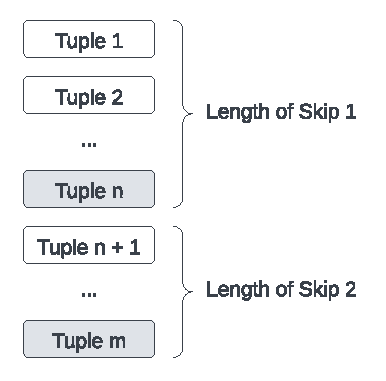
\includegraphics[height=5cm]{figure1.pdf}
            \caption{Example of two skips with different lengths}
        \end{wrapfigure}
        But deciding for every tuple separately using the probability method can be rather expensive. Therefore, the algorithm generates a length of a skip instead. The length is stored with some additional metadata in skip node and can be used to determine how many tuples should be skipped until the next reservoir tuple. A skip node that contains valid data is also called a skip. To determine whether a tuple is a reservoir tuple or not using the skip length is very cheap. First the skip length needs to be decremented by one and if the length reached zero the current tuple is a reservoir tuple and a new one skip needs to be generated. Figure one shows an example for two skips. The white tuples are skipped and the gray tuples are reservoir tuples.

        % Multithreaded skip nodes
        Hence, the skips are already stored in self contained nodes, these nodes can easily be distributed among multiple threads. Only the generation and distribution needs to be synchronized, 
        % Explain ownership
        once a thread owns a node no more synchronization is required and the thread can work independently. Every thread receives an independent stream of tuples that should be inserted and therefore also sampled. The amount of tuples is unknown and each thread could stop receiving tuples at any moment.

        % Preallocation
        To ensure the constant use of memory it is necessary that the maximum amount of threads that can be used for inserting is known when the algorithm is initialized. In consequence all skip nodes can be preallocated, one for every thread and one additional node as reserve (the reason for the reserve node is explained later on). Hence, a pointer to a skip node can simply be an index into the node array.

        % States of a skip node
        \begin{figure}[h]
            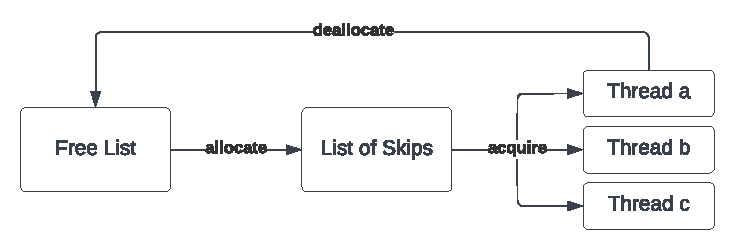
\includegraphics[height=3.5cm]{figure2.pdf}
            \caption{States of a skip node and the transitions between the states}
        \end{figure}
        One additional field that is stored in every skip node, is a successor pointer. This pointer can be used to arrange nodes in a singly linked list. There are three states a skip node can be in, initially all nodes are in the free list. The free list contains all nodes that are currently not used by any thread and nodes that do not contain valid data. If a skip should be generated a node needs to be allocated, thus it needs to be removed from the free list and the data of skip can be stored in this node. Afterwards the node is added to the list of skips (LOS). The LOS contains all nodes that store a valid skip, but are not currently owned by a thread. Additionally the LOS should always contain at least on skip. When a thread needs acquire a new skip, it can pop the first item of the LOS. Afterwards the thread might need to generate a new skip to ensure that the LOS is not empty. Figure 2 illustrates the lifecycle of a skip node.

    \subsection{Sampling while inserting}

    \section{Example}
        % An example who the algorithm works (similar to one in the OG)
        This is an example.

    \section{Evaluation}
        % Are all requirements met
        % Tables from the OG
        This is the evaluation.

\end{document}